\documentclass{article}
\usepackage{amsmath}

\usepackage{graphicx}
\usepackage{hyperref}
\usepackage{float}
\usepackage{csvsimple}
\usepackage{subcaption}

\graphicspath{./images/}

\title{Rapport de laboratoire: \\Intelligence Artificielle}
\author{Matthias Léonard et Dawid Krasowski}
\date{2022/2023}

\begin{document}
\maketitle

\begin{figure}[h]
    \centering
    
\includegraphics[scale=0.15]{./images/Logo ECAM.png}

\end{figure}


\paragraph{Superviseur :} Monsieur HASSELMANN Ken



\pagebreak
\tableofcontents
\pagebreak
\section{Introduction}

    Dans le cadre des laboratoires d'intelligence artificielle dispensé à l'ECAM en 2ème Master en ingénieur informatique.
Sous la supervision de Monsieur HASSELMANN notre projet se base sur la recherche de fraude à la carte bancaire.
Nous travaillons sur un jeu de données de transactions bancaires issues d'Ouganda 
ces données on été fournis lors d'une compétition Xente de 2019.\\ \url{https://zindi.africa/competitions/xente-fraud-detection-challenge} \\

Notre projet est disponible sur GitHub à l'adresse suivante :\\ \url{https://github.com/LeTouristeDeLECAM/Lab_AI_Fraud_Detection} \\
Pour des questions de propriété et droit les données ne sont pas disponibles sur GitHub.


\section{Présentation des données}
\subsection{Description des données}

% Added description table 
\begin{table}[h]
\centering
\csvautotabular{../../Data/Xente_Variable_Definitions.csv}
\caption{Description des données}
\end{table}

\subsection{identification des Features}
Dans un premier temps nous cherchons à identifier les features qui vont nous permettre de créer un modèle de prédiction de fraude.\\

Nous pouvons observer que certaines données ne sont pas utile pour obtenir un modèle. 
Nous décidons de supprimer les colonnes suivantes :
%list 
\begin{itemize}
    \item CurrencyCode : Toutes les transactions sont en UGX soit en Shilling Ougandais.
    \item CountryCode : Toutes les transactions sont en Ouganda.
\end{itemize} 
Nous pouvons également imaginer à première vue que les données Amount et Value sont similaires.
Néanmoins suite à une analyse: \\ \\
%Italique
\emph{diff = test2["Amount"] - abs(test2["Value"])\\diff.describe()}\\

nous pouvons observer que les deux colonnes ne sont pas totalement identiques.\\
% ajout de la table csv
\begin{table}[h]
    \centering
    \csvautotabular{./images/Amout_Value_description.csv}
    \caption{Description statistique de la différence entre Amount et Value}
        
 \end{table}

Nous avons décidé de garder les données Amount et Value. Car sur les 193 fraudes que comporte le jeu de données, 
17  fraudes sont réalisé quand Amount et Value sont différents (8,8\%).\\

\paragraph{Features à supprimer :}
% figure import 
\begin{figure}[h]
    \centering
    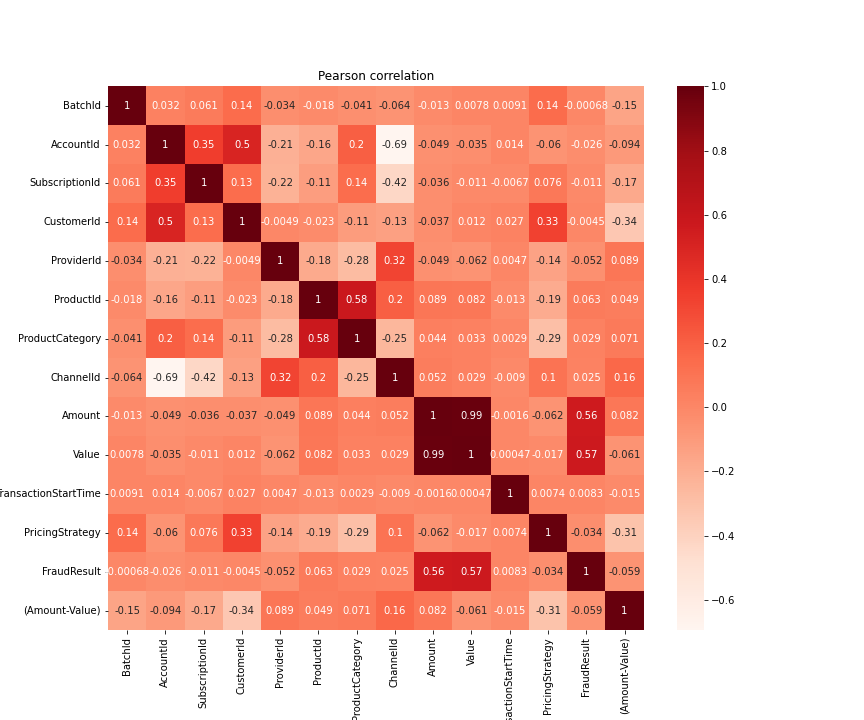
\includegraphics[scale=0.4]{./images/correlation_pearson.png}
    \caption{Corrélation de Pearson entre les features} 
\end{figure}





Nous pouvons observer que productCategory et productID sont fortement corrélés.
il en est de même pour amount et value.\\

Pour pousuivre notre analyse nous réalisons une analyse en composante principale (ACP) sur les données.\\
Cette analyse nous permet de réduire la dimensionnalité de nos données et identifier les données qui sont les plus importantes.\\

\subsection{Optimization de la Feature TransactionStartTime}

La feature TransactionStartTime est un horodatage, les données disponibles s'étendent de 15 novembre 2018 au 13 février 2019,
Nous pouvons difficilement découper cette transformer cette feature pour déterminer un comportement sur une période tel que les mois ou les jours.\\
Nous avons décidé d'utiliser uniquement l'heure de la transaction pour identifier un comportement une tendance de comportement. \\

% figure import
\begin{figure}[h]
    \centering
    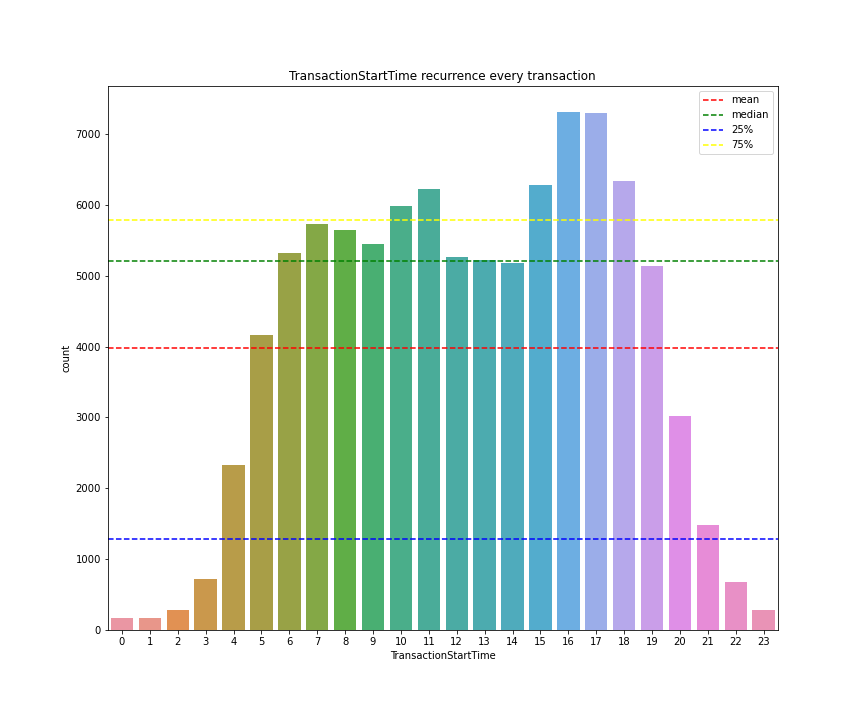
\includegraphics[scale=0.2]{./images/TransactionStartTime_recurrence_every_transaction.png}
    \caption{Distribution des transactions en fonction de l'heure}

    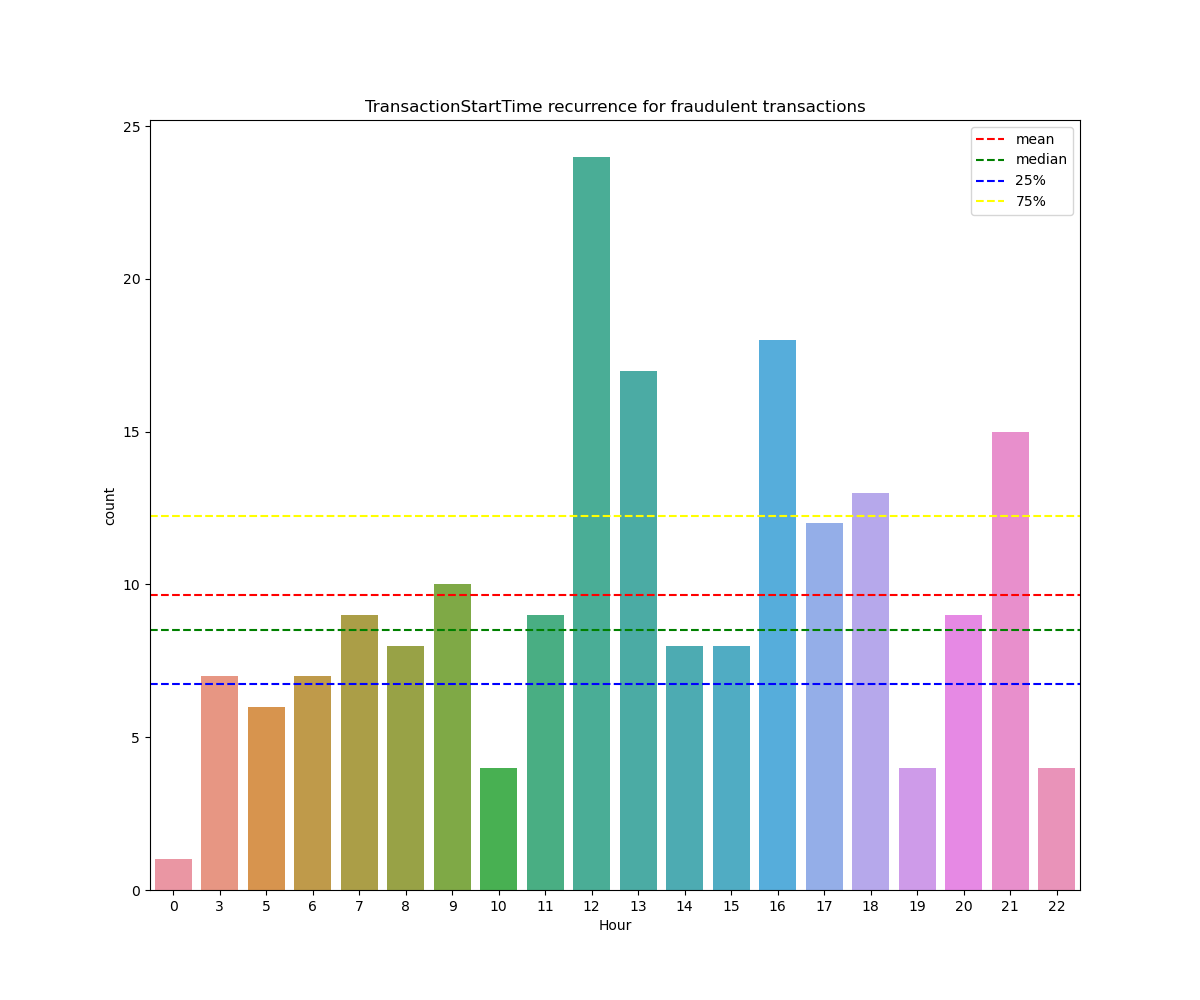
\includegraphics[scale=0.2]{./images/TransactionStartTime_recurrence_fraud.png}
    \caption{Distribution des transactions frauduleuses en fonction de l'heure}
    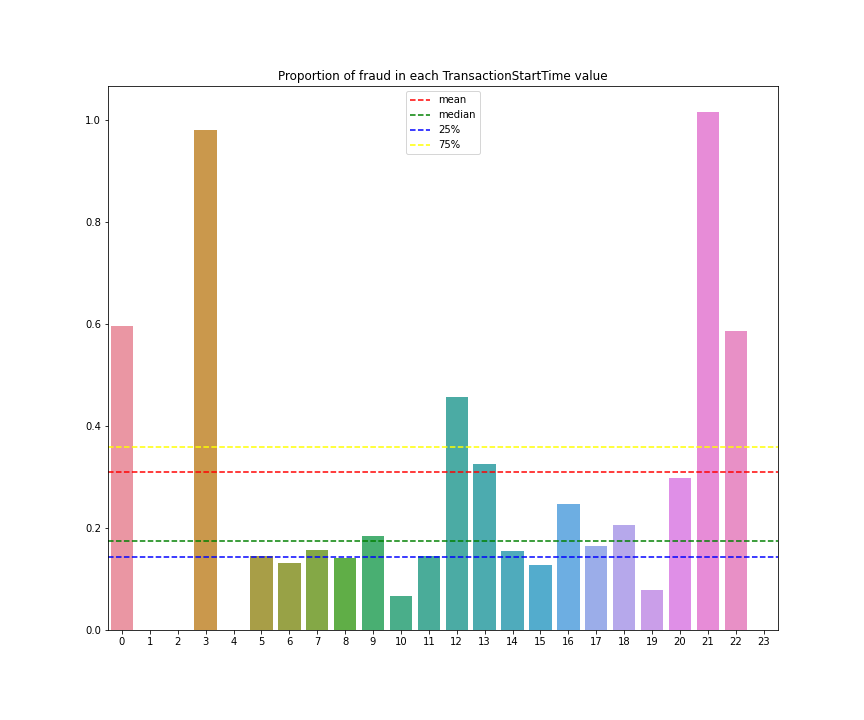
\includegraphics[scale=0.2]{./images/TransactionStartTime_proportion_fraud.png}
    \caption{Distribution du rapport des transactions frauduleuses en fonction de l'heure}
\end{figure}


\begin{figure}
  \begin{subfigure}{\linewidth}
  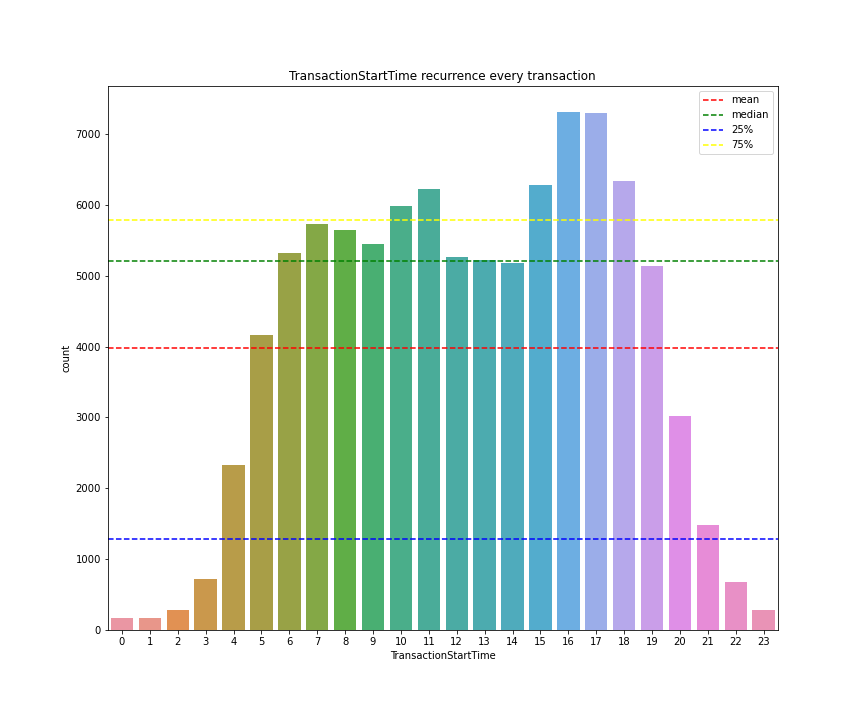
\includegraphics[width=.3\linewidth]{./images/TransactionStartTime_recurrence_every_transaction.png}\hfill
  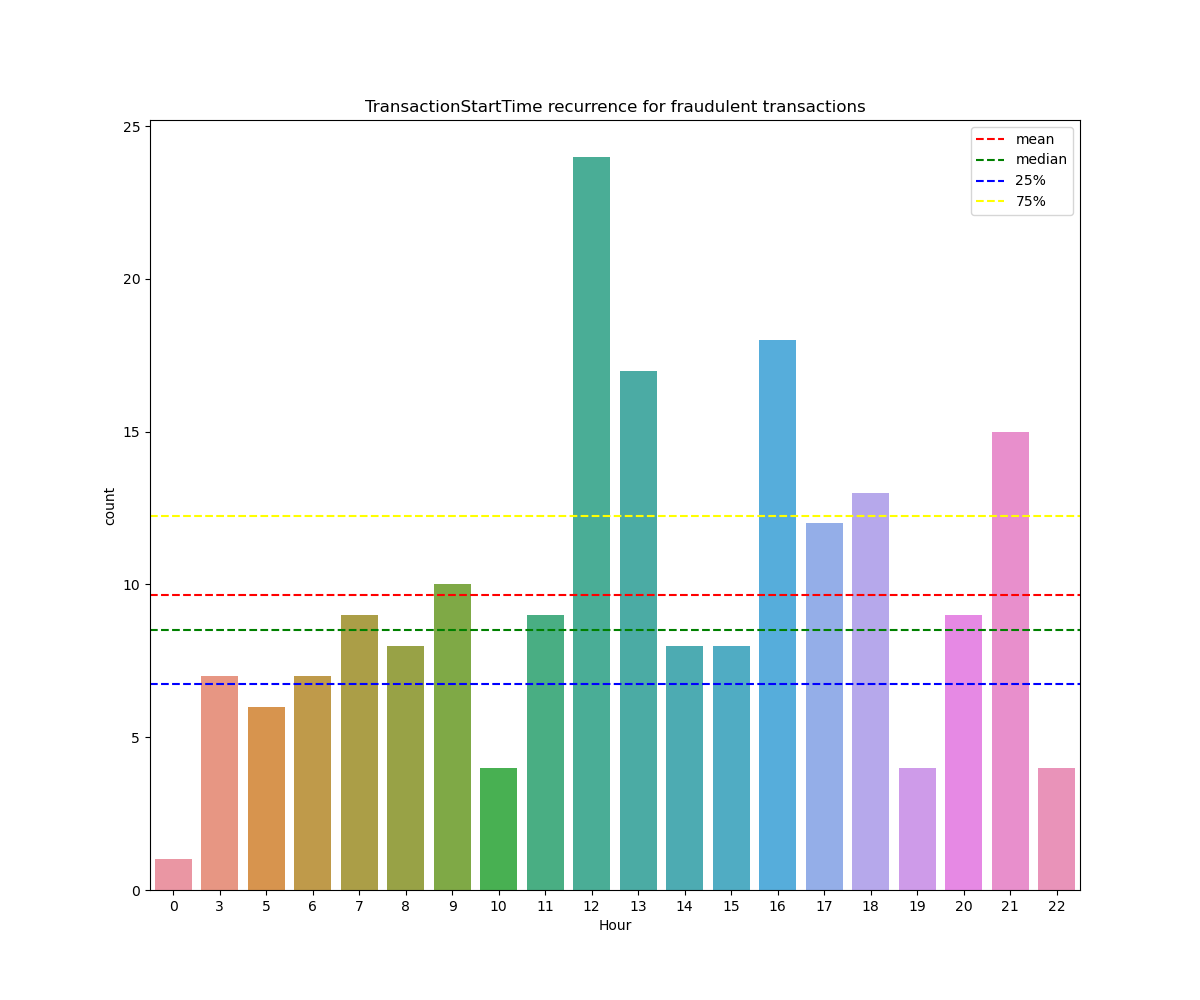
\includegraphics[width=.3\linewidth]{./images/TransactionStartTime_recurrence_fraud.png}\hfill
  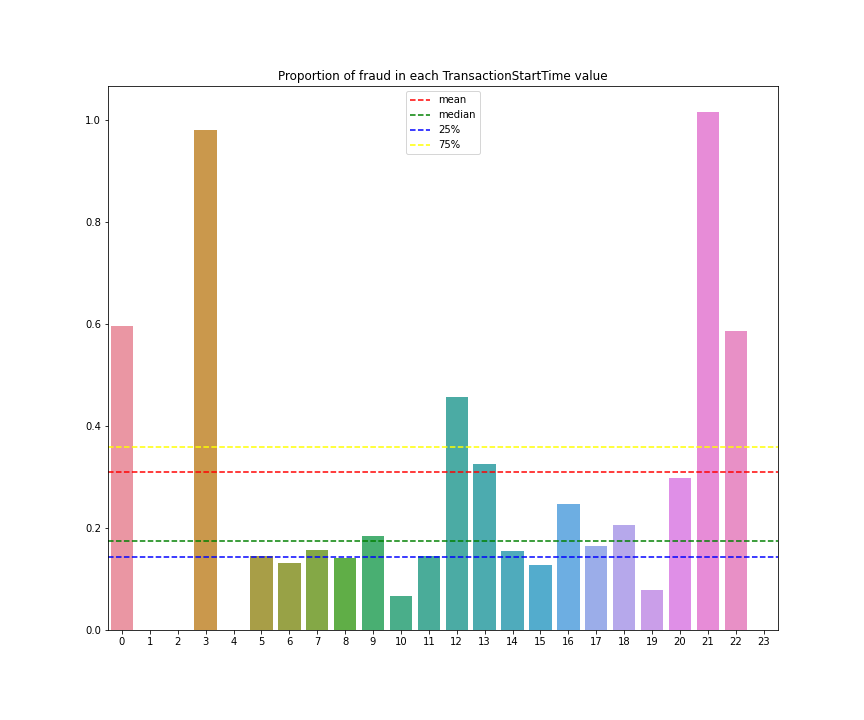
\includegraphics[width=.3\linewidth]{./images/TransactionStartTime_proportion_fraud.png}
  \end{subfigure}\par\medskip
  
  \caption{Some grouped images}
\end{figure}


En observant les graphiques ci-dessus nous pouvons observer que la distribution des transactions suit une courbe de gauss avec un creux durant le temps de midi. Nous observons que la distribution des transactions frauduleuses ne suit pas  exactement la même distribution, 
La distribution semble plus uniforme est semble moins suivre une courbe de gauss avec un plus grand écart-type.\\
Pour donner plus de sens au observation nous nous intéressons à la proportion de transaction frauduleuse en fonction de l'heure.\\
Nous pouvons observer que la proportion de transaction frauduleuse est plus élevée durant la nuit et le temps de midi.\\
Nous avons décidé de transformer la feature TransactionStartTime en une feature catégorielle:\\
% list 
\begin{itemize}
    \item 1: Morning 04h00 - 11h59
    \item 2: Lunch 12h00 - 13h59
    \item 3: Afternoon 12h00 - 19h59
    \item 4: Night 20h00 - 03h59
\end{itemize}

Observons la distribution des transactions avec la nouvelle feature.\\

% figure import
\begin{figure}[h]
    \begin{subfigure}{\linewidth}
        \centering
        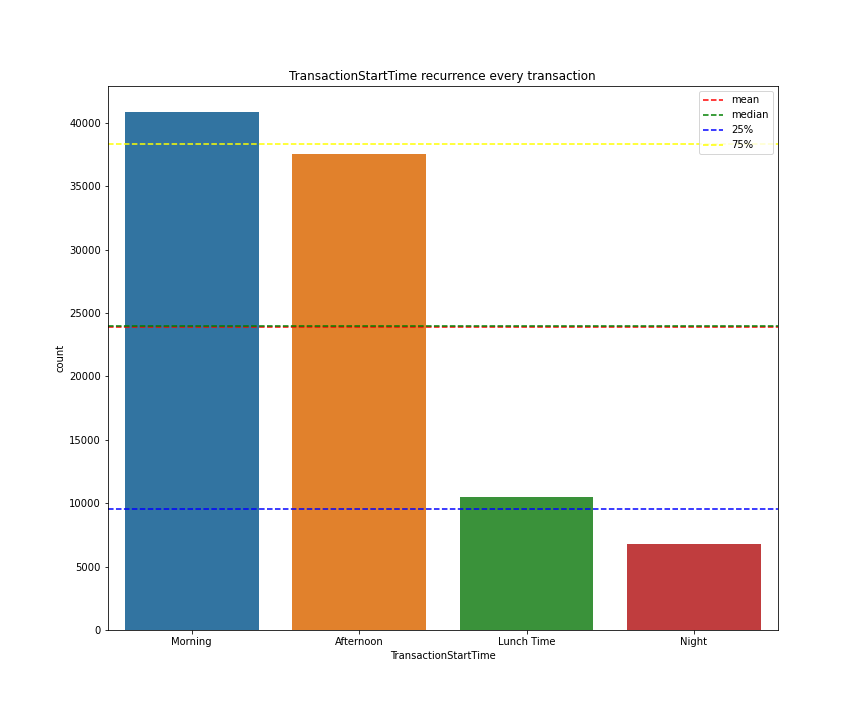
\includegraphics[width=.3\linewidth]{./images/TransactionStartTime_recurrence_every_transaction_new_feature.png}\hfill
        %\caption{Distribution des transactions en fonction de l'heure}
        
        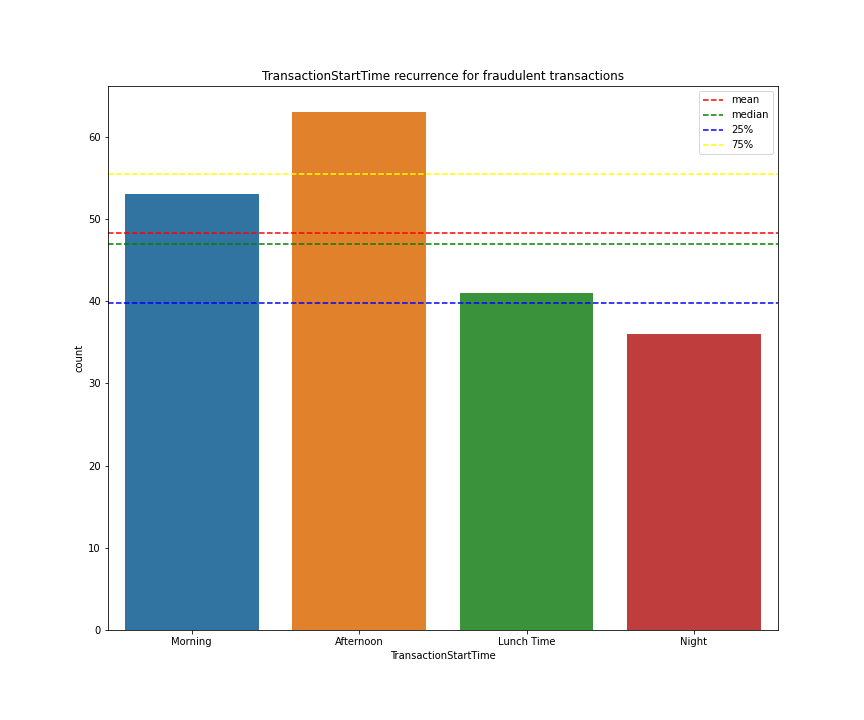
\includegraphics[width=.3\linewidth]{./images/TransactionStartTime_recurrence_fraud_new_feature.png}\hfill
        %\caption{Distribution des transactions frauduleuses en fonction de l'heure}
        
        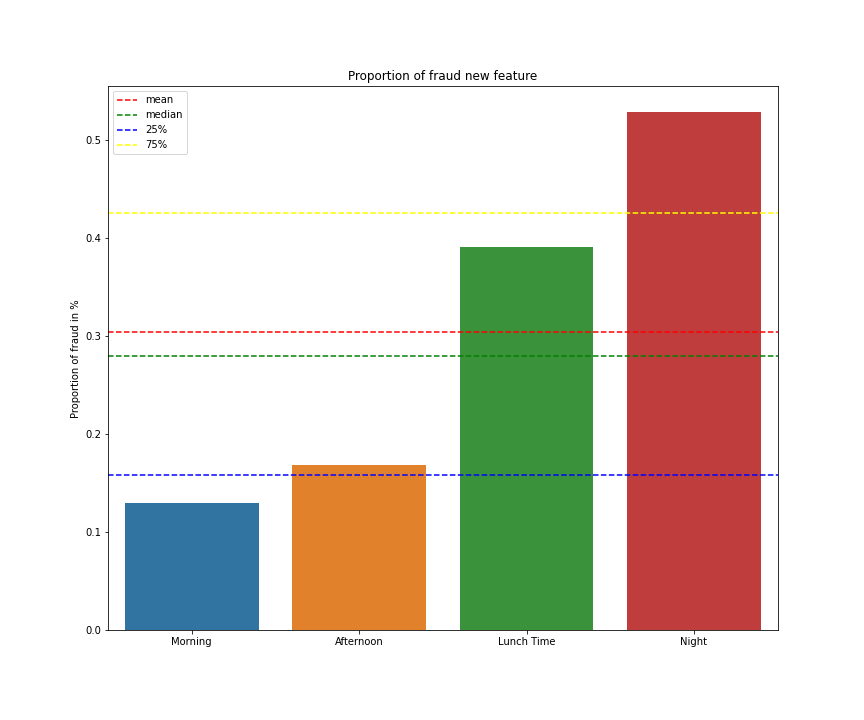
\includegraphics[width=.3\linewidth]{./images/TransactionStartTime_proportion_fraud_new_feature.png}
        %\caption{Distribution du rapport des transactions frauduleuses en fonction de l'heure}

    \centering
    \end{subfigure}
    

\end{figure}



\begin{figure}
    \subfloat[]{%
    \begin{minipage}{\linewidth}
    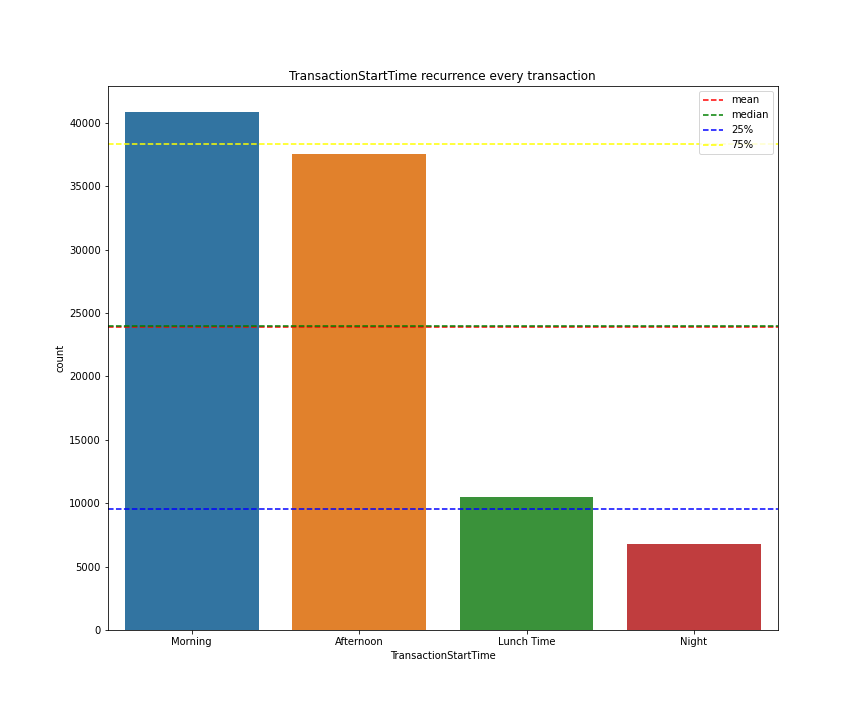
\includegraphics[width=.3\linewidth]{./images/TransactionStartTime_recurrence_every_transaction_new_feature.png}\hfill
    %\caption{}
    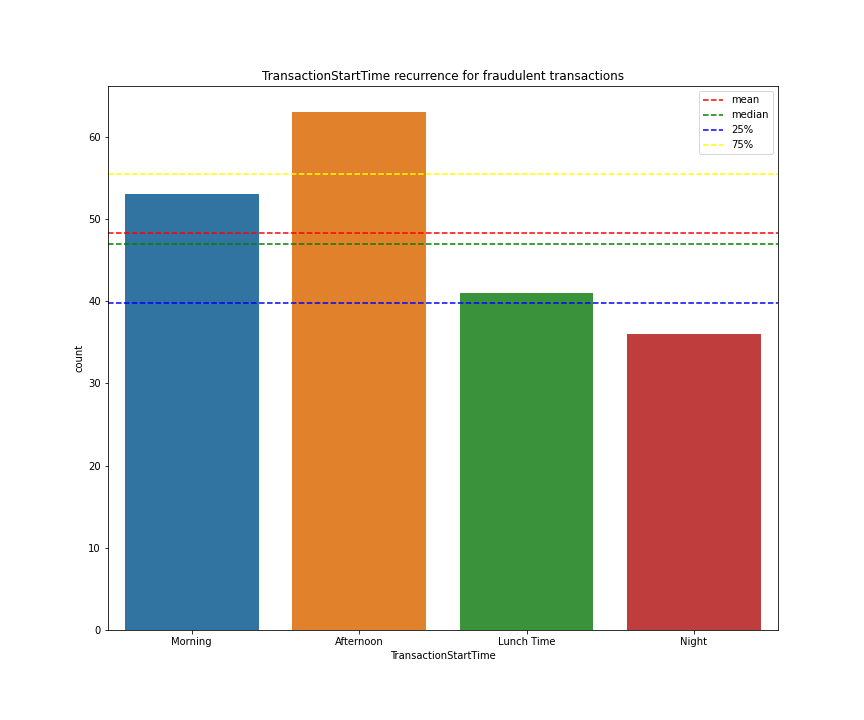
\includegraphics[width=.3\linewidth]{./images/TransactionStartTime_recurrence_fraud_new_feature.png}\hfill
    %\caption{}
    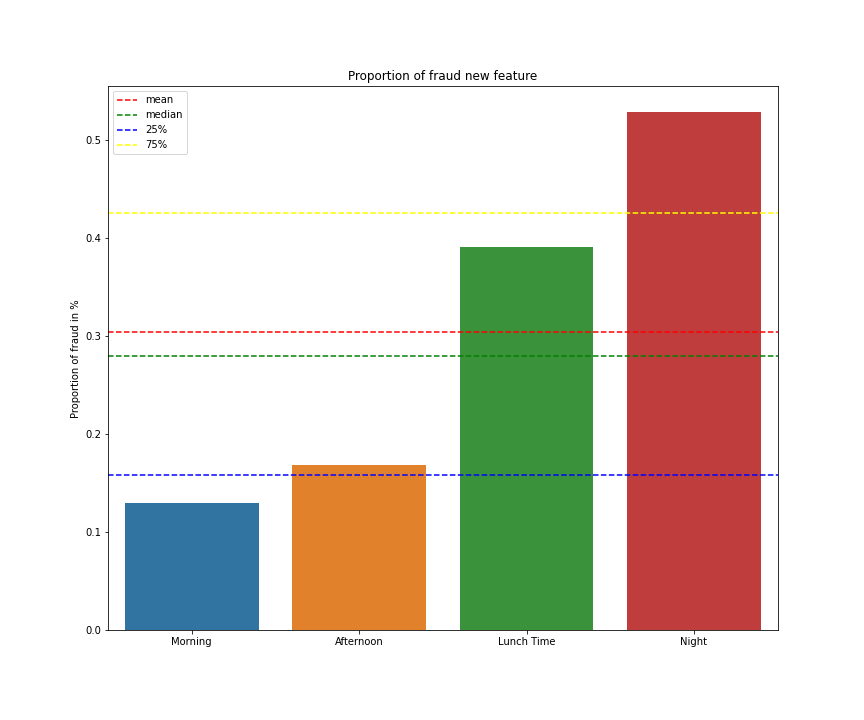
\includegraphics[width=.3\linewidth]{./images/TransactionStartTime_proportion_fraud_new_feature.png}%
    %\caption{}
    \end{minipage}%
    }
  
    \caption{Distribution des transactions en fonction de l'heure: toutes (a), frauduleuses (b), proportion frauduleuses (c)}
  \end{figure}

Avec la transformation de la feature TransactionStartTime en une feature catégorielle nous observons que la proportion de transaction frauduleuse est plus élevée durant la nuit et le temps de midi.\\
Avec cette transformation nous avons accrue l'importance de cette features pour notre modèle.\\


\section{Unbalanced Data}
Pour palier au problème de données déséquilibrées il nous est possible de travailler avec plusieurs méthodes.
Nous pouvons utiliser des méthodes d'Oversampling ou d'Undersampling ou encore une combinaison des deux.\\
Nous avons décider d'utiliser la méthode easy ensemble qui est une méthode d'undersampling aléatoire coupler avec un algorithme de boosting.
Conceptuellement cette méthode consiste à créer plusieurs sous-ensembles de données en sous-échantillonnant la classe majoritaire.
Nous utilisons Adaboost comme classifieur pour chaque sous-ensemble de données, Nous utiliseons également comparons également avec l'algorithme Gradient Boosting Classifier.
Nos résultats sont présentés dans le tableau ci-dessous.\\
%italic 
%\textit{EasyEnsembleClassifier(n_estimators=20, estimator=AdaBoostClassifier() , random_state=42, n_jobs=-1, verbose=0)}
%\textit{EasyEnsembleClassifier(n_estimators=50, estimator=GradientBoostingClassifier() , random_state=42, n_jobs=-1, verbose=0 )}
%\textif{EasyEnsembleClassifier(n_estimators=20, estimator=AdaBoostClassifier(), sampling_strategy=0.25 , random_state=42, n_jobs=-1, verbose=0)}

% tableau
\begin{table}[h]
    \centering
    \begin{tabular}{|c|c|c|c|}
        \hline
         & Accuracy & Recall & F1-Score \\
        \hline
        AdaBoost   & 0.9995 & 0.8571 & 0.8571 \\
        %n_estimators=20 & 0 & 0 & 0\\
        %sampling_strategy=0.25 & 0 & 0 & 0 \\
        \hline
        AdaBoost & 0.9995 & 0.8571 & 0.8571 \\
        \hline
        Gradient Boosting & 0.9995 & 0.8571 & 0.8571 \\
        \hline
    \end{tabular}
    \caption{Résultats de la méthode Easy Ensemble Classifier}

\end{table}

\section{Conclusion}
Nous avons observé une diminution de la divergence.
\end{document}
